In the cluster \textbf{Model}, there are two important parent classes: Class \texttt{PLAYER} and class \texttt{BRAIN}. \texttt{PLAYER} is the parent of \texttt{FLAT\_HUNTER} and \texttt{ESTATE\_AGENT}, and \texttt{BRAIN} is the parent of \texttt{HUMAN}, \texttt{FLAT\_HUNTER\_BOT} and \texttt{ESTATE\_AGENT\_BOT}. These \textbf{Model} classes describe the internal representation of ``real world'' objects. Here is a description of some of these classes.

\begin{itemize}
  \item{\textbf{PLAYER}: Class \texttt{PLAYER} knows the basic things one needs to know about a player of \emph{Flat Hunt}, like how many tickets he got left. It features the commands \textit{play} and \textit{move} and has either a \texttt{HUMAN} or a \texttt{BOT} brain.}
  \item{\textbf{ESTATE\_AGENT}: This is one of the two heirs of class \texttt{PLAYER}. It has some additional information that is special for an estate agent player like knowing where he last showed himself.}
  \item{\textbf{BRAIN}: Class \texttt{BRAIN} includes the intelligence to choose the next move.}
\end{itemize}

\begin{figure}[h]
\centerline{\hbox{  
  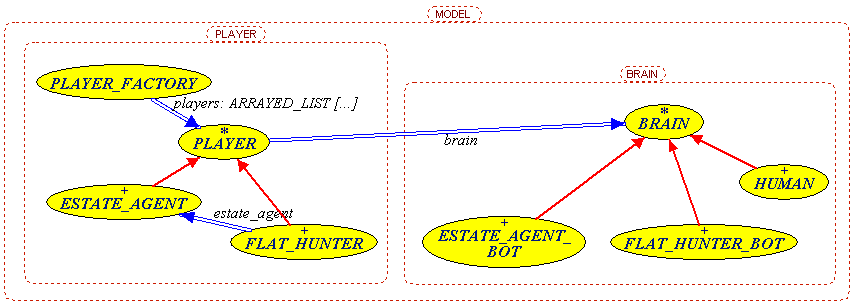
\includegraphics[width=135mm]{model}
  }}
\caption{Diagram of the Model Cluster}
\label{modeldiagram}
\end{figure}
